\documentclass[journal]{IEEEtran}

\usepackage{ifpdf}
\usepackage{cite}
\usepackage{acronym}
\usepackage{url}
\usepackage{graphicx}
\usepackage{tabularx}
\usepackage{amsmath}
\usepackage{algorithm}
\usepackage{algpseudocode}
\usepackage{tikz}
\usepackage{subfig}
\usetikzlibrary{automata, positioning, arrows.meta}
\DeclareGraphicsExtensions{.pdf,.jpeg,.png}
\renewcommand\tabularxcolumn[1]{m{#1}}

\hyphenation{op-tical net-works semi-conduc-tor}

\acrodef{IoT}{Internet of Things}
\acrodef{LoRa}{Long Range}
\acrodef{LoRaWAN}{Long Range Wide Area Network}
\acrodef{SPI}{Serial Peripheral Interface}
\acrodef{RSSI}{Received Signal Strength Indicator}
\acrodef{CRC}{Cyclic Redundancy Check}
\acrodef{LoS}{Line-of-Sight}
\acrodef{NLoS}{Non-Line-of-Sight}
\acrodef{ADR}{Adaptive Data Rate}
\acrodef{UAV}{Unmanned Aerial Vehicle}
\acrodef{LAMP}{LoRa Adaptive Multipacket Protocol}
\acrodef{SACK}{Selective Acknowledgment}
\acrodef{ARQ}{Automatic Repeat Request}
\acrodef{3WHS}{3-Way Handshake}
\acrodef{HAL}{Hardware Abstraction Layer}
\acrodef{TDD}{Test-Driven Development}
\acrodef{FEC}{Forward Error Correction}
\acrodef{LPWAN}{Low-Power Wide-Area Network}
\acrodef{MPLR}{Multi-Packet LoRa}
\acrodef{GPIO}{General-Purpose Input/Output}
\acrodef{FIFO}{First-In, First-Out}
\acrodef{ETSI}{European Telecommunications Standards Institute}
\acrodef{ERP}{Effective Radiated Power}
\acrodef{SNR}{Signal-to-Noise Ratio}

\begin{document}

\title{Supplementary Material for LAMP: A Selective-ACK Transport Protocol for Reliable Bulk Data Transmission over LoRa Networks}

\author{Alessandro~Monticelli,~\IEEEmembership{Student~Member,~IEEE}%
\thanks{A. Monticelli is with the Department of Information Engineering, University of Pisa, Italy (e-mail: alessandro.monticelli@ing.unipi.it).}}

\maketitle

\begin{abstract}
This supplementary document provides extended implementation details, architectural state machines, and secondary parametric simulation blocks supporting the main manuscript ``LAMP: A Selective-ACK Transport Protocol for Reliable Bulk Data Transmission over LoRa Networks''. Specifically, we document: (i) the preliminary commercial transceiver proof-of-concept and its architectural lessons; (ii) the detailed Hardware Abstraction Layer (HAL) architecture on ESP32-S3 and desktop Unity test harness; (iii) formal finite state machine specifications for session lifecycle and data transfer; and (iv) extended ns-3 simulation studies evaluating message size scaling up to 62.2~kB (Block~F), asymmetric acknowledgment loss sensitivity (Block~G), retransmission poll rule ablation (Block~H), and additional propagation channel profiles (Rural, Water, Static).
\end{abstract}

\begin{IEEEkeywords}
LoRa, SACK, transport protocol, embedded systems, HAL, state machines, sensitivity analysis.
\end{IEEEkeywords}
\acresetall

\section{Preliminary Proof of Concept: Commercial UART Transceivers}
\label{sec:supp_poc}
Prior to developing the native C++17 LAMP stack on Semtech SX1262 transceivers, an initial proof-of-concept was developed and evaluated using commercial Ebyte E220-series LoRa modules. These modules encapsulate physical-layer modulation behind an internal microcontroller running proprietary AT-command firmware accessible over an asynchronous UART interface.

While initial lab tests confirmed the basic feasibility of transport fragmentation over LoRa physical links, the trial exposed three critical architectural bottlenecks that motivated the ground-up redesign of LAMP:
\begin{enumerate}
  \item \textbf{Opaque PHY and Inflexible MAC Control}: The proprietary internal firmware prevented direct access to raw baseband parameters, fine-grained symbol timing, carrier-activity detection (CAD), and exact FIFO interrupt timestamps, making deterministic timeout scheduling and half-duplex turnaround guard times impossible to guarantee.
  \item \textbf{Inflated Protocol Overhead}: The vendor-mandated framing structure introduced substantial packet encapsulation bloat, reducing the net application payload capacity per frame and significantly increasing channel time-on-air (ToA).
  \item \textbf{Absence of Receiver Feedback and Repair}: The commercial module firmware offered no native selective acknowledgment or sliding-window ARQ mechanisms, forcing early prototype firmware to resort to crude unacknowledged bursts or inefficient Stop-and-Wait retries.
\end{enumerate}

These empirical findings motivated the complete transition to the open-source Semtech SX126x architecture driven via RadioLib and decoupled by a clean Hardware Abstraction Layer (HAL).

\section{Hardware Abstraction Layer and Implementation Architecture}
\label{sec:supp_hal}

\subsection{Centralized Configuration and Parameter Decoupling}
To eliminate hardcoded constants and enable deterministic tuning across heterogeneous embedded targets, all protocol operational parameters are centralized within a compile-time configuration namespace (\texttt{LoRaMultiPacketConfig}):
\begin{itemize}
  \item \textbf{Memory and Concurrency Bounds}: Governs maximum concurrent reassembly sessions (\texttt{MAX\_CONCURRENT\_SESSIONS} = 10, reducible on memory-constrained microcontrollers), physical FIFO buffer bounds (\texttt{PHY\_BUFFER\_SIZE} = 256~bytes, matching transceiver hardware FIFO limits), and completed sequence deduplication depth (\texttt{MAX\_COMPLETED\_HISTORY} = 16).
  \item \textbf{Timing and Retransmission Policies}: Configures the default retry ceiling ($R_{\mathrm{max}} = 5$), minimum SACK timeout floor ($T_{\min} = 1000$~ms), safety multiplier ($\alpha = 1.5$), and half-duplex switching guard ($\delta_{\mathrm{sw}} = 25$~ms).
  \item \textbf{Session Lifecycle Thresholds}: Defines handshake initiation timeouts (\texttt{DEFAULT\_SYN\_TIMEOUT\_MS} = 3000~ms), connection inactivity teardown periods (\texttt{DEFAULT\_CONN\_INACTIVITY\_TIMEOUT\_MS} = 15000~ms), and the reassembly inactivity limit, measured from the last chunk received: the larger of \texttt{PRUNE\_TIMEOUT\_MS} = 15000~ms and $(R_{\mathrm{max}}+1)$ SACK timeouts.
\end{itemize}

\subsection{Hardware Abstraction Layer (\ac{HAL}) Interface}
The core transport logic communicates exclusively through abstract interfaces (\texttt{IRadio} and \texttt{IPlatform}). On physical nodes, \texttt{EspHal} wraps ESP32-S3 hardware resources:
\begin{itemize}
  \item \textbf{SPI Bus Access}: High-speed SPI transfers (up to 16~MHz) for register configuration and FIFO packet buffering to the Semtech SX1262.
  \item \textbf{GPIO Interrupt Management}: Hardware interrupt dispatch for NSS, RST, BUSY, and DIO1 (packet transmission and reception completion triggers).
  \item \textbf{Monotonic Timing}: High-resolution platform timers backed by \texttt{esp\_timer\_get\_time()} providing microsecond-level precision decoupled from RTOS tick scheduling.
\end{itemize}

\subsection{Host-Based Unit Testing Suite}
Following a test-driven development (TDD) discipline, the protocol core is verified on a desktop host environment using the Unity test framework within PlatformIO (72 native unit tests), executing without hardware-in-the-loop dependencies:
\begin{enumerate}
  \item \textit{Modbus CRC-16 Verification}: Frame integrity calculation across variable-length headers and padded chunk payloads.
  \item \textit{Reassembly State Engine}: Dynamic bitmap updates, out-of-order chunk reassembly, and duplicate suppression.
  \item \textit{Deterministic Pruning}: Verification that abandoned or stale sessions are evicted when inactivity timers expire.
  \item \textit{Concurrency Keys}: Proving that multiple active senders with identical message IDs remain isolated through $(\mathtt{srcAddr}, \mathtt{messageId})$ dual indexing.
  \item \textit{Simultaneous Open \& Tie-Breaking}: Confirming deterministic resolution when two nodes initiate concurrent 3-way handshakes.
\end{enumerate}

\section{Finite State Machine Formal Specifications}
\label{sec:supp_fsm}

Fig.~\ref{fig:supp_state_machines} details the formal finite state machines governing the connection lifecycle and data transfer engines within LAMP.

\begin{figure*}[htpb]
\centering
\subfloat[Connection Session Lifecycle FSM (Stateful vs. Stateless)]{%
  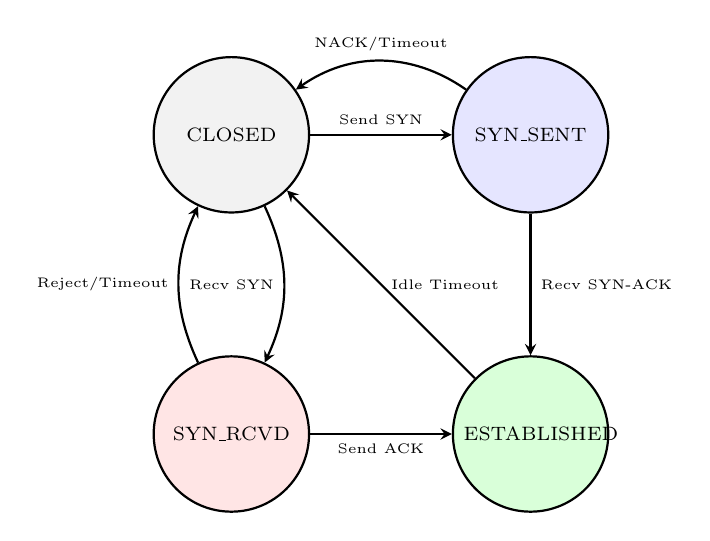
\begin{tikzpicture}[->, >=stealth, thick, auto, font=\scriptsize, transform shape, every node/.style={align=center}]
    \node[draw, circle, fill=gray!10, minimum size=1.7cm, text width=1.7cm] (closed) at (0,0) {CLOSED};
    \node[draw, circle, fill=blue!10, minimum size=1.7cm, text width=1.7cm] (synsent) at (3.8,0) {SYN\_SENT};
    \node[draw, circle, fill=red!10, minimum size=1.7cm, text width=1.7cm] (synrcvd) at (0,-3.8) {SYN\_RCVD};
    \node[draw, circle, fill=green!15, minimum size=1.7cm, text width=1.7cm] (established) at (3.8,-3.8) {ESTABLISHED};

    \path
      (closed) edge node[above, font=\tiny] {Send SYN} (synsent)
      (closed) edge[bend left=25] node[left, font=\tiny] {Recv SYN} (synrcvd)
      (synsent) edge node[right, font=\tiny] {Recv SYN-ACK} (established)
      (synrcvd) edge node[below, font=\tiny] {Send ACK} (established)
      (synsent) edge[bend right=35] node[above, sloped, font=\tiny] {NACK/Timeout} (closed)
      (synrcvd) edge[bend left=25] node[left, font=\tiny] {Reject/Timeout} (closed)
      (established) edge node[right, font=\tiny] {Idle Timeout} (closed);
  \end{tikzpicture}%
  \label{fig:supp_fsm_connection}%
}\hfill
\subfloat[Data Transfer \& SACK-ARQ FSM (Reliable vs. Unreliable)]{%
  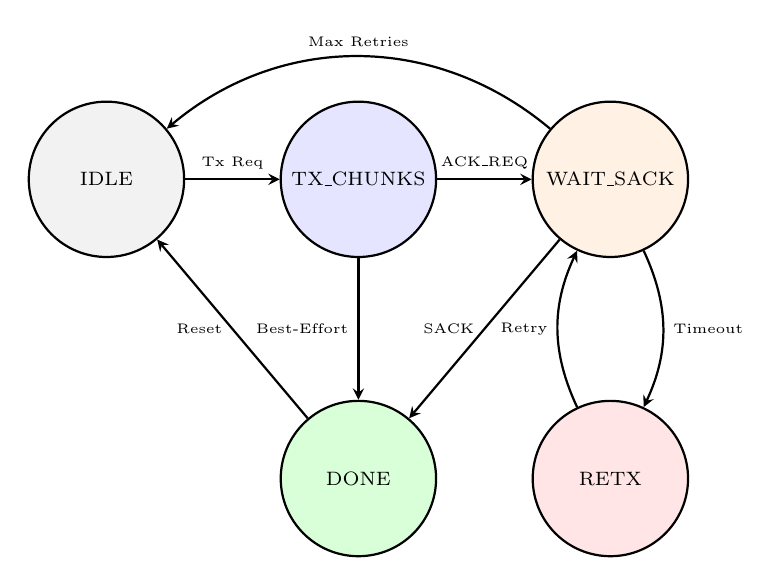
\begin{tikzpicture}[->, >=stealth, thick, auto, font=\scriptsize, transform shape, every node/.style={align=center}]
    \node[draw, circle, fill=gray!10, minimum size=1.7cm, text width=1.7cm] (idle) at (0,0) {IDLE};
    \node[draw, circle, fill=blue!10, minimum size=1.7cm, text width=1.7cm] (send) at (3.2,0) {TX\_CHUNKS};
    \node[draw, circle, fill=orange!10, minimum size=1.7cm, text width=1.7cm] (wait) at (6.4,0) {WAIT\_SACK};
    \node[draw, circle, fill=red!10, minimum size=1.7cm, text width=1.7cm] (retransmit) at (6.4,-3.8) {RETX};
    \node[draw, circle, fill=green!15, minimum size=1.7cm, text width=1.7cm] (completed) at (3.2,-3.8) {DONE};

    \path
      (idle) edge node[above, font=\tiny] {Tx Req} (send)
      (send) edge node[above, font=\tiny] {ACK\_REQ} (wait)
      (send) edge node[left, font=\tiny] {Best-Effort} (completed)
      (wait) edge[bend left=25] node[right, font=\tiny] {Timeout} (retransmit)
      (retransmit) edge[bend left=25] node[left, font=\tiny] {Retry} (wait)
      (wait) edge node[left, font=\tiny] {SACK} (completed)
      (wait) edge[bend right=40] node[above, sloped, font=\tiny] {Max Retries} (idle)
      (completed) edge node[left, font=\tiny] {Reset} (idle);
  \end{tikzpicture}%
  \label{fig:supp_fsm_datatransfer}%
}
\caption{Finite State Machine (FSM) specifications for connection session lifecycle and data transfer modes.}
\label{fig:supp_state_machines}
\end{figure*}

\subsection{Protocol Sequence Interactions}
Fig.~\ref{fig:supp_3whs_sequence} and Fig.~\ref{fig:supp_data_transfer_sequence} illustrate the detailed message interaction flows for connection establishment, rejection handling, and SACK-ARQ selective repair.

\begin{figure*}[htpb]
\centering
\subfloat[Successful 3-Way Handshake (3WHS) with Metadata Negotiation]{%
  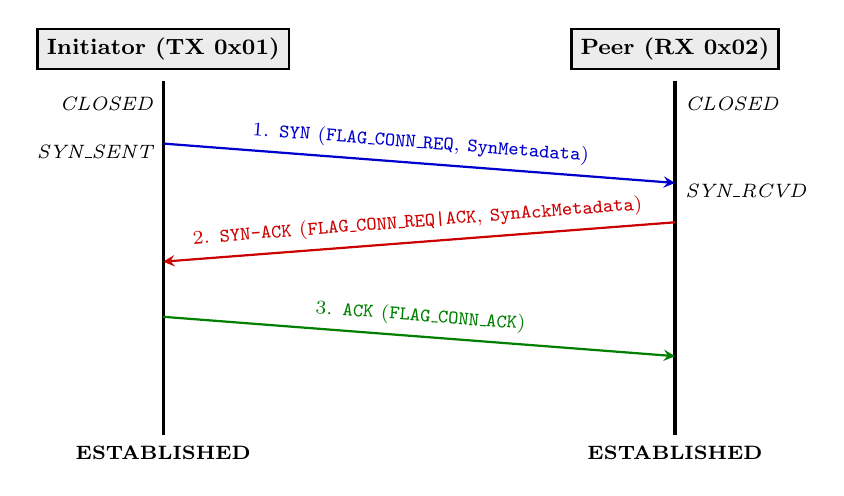
\begin{tikzpicture}[>=stealth, thick, font=\footnotesize]
    \draw[very thick] (0,0) -- (0,-4.5) node[below, font=\scriptsize\bfseries] {ESTABLISHED};
    \draw[very thick] (6.5,0) -- (6.5,-4.5) node[below, font=\scriptsize\bfseries] {ESTABLISHED};

    \node[draw, rectangle, fill=gray!15, minimum width=2.2cm, minimum height=0.5cm] at (0,0.4) {\textbf{Initiator (TX 0x01)}};
    \node[draw, rectangle, fill=gray!15, minimum width=2.2cm, minimum height=0.5cm] at (6.5,0.4) {\textbf{Peer (RX 0x02)}};

    \node[left, font=\scriptsize\itshape] at (0,-0.3) {CLOSED};
    \node[right, font=\scriptsize\itshape] at (6.5,-0.3) {CLOSED};
    \node[left, font=\scriptsize\itshape] at (0,-0.9) {SYN\_SENT};
    \node[right, font=\scriptsize\itshape] at (6.5,-1.4) {SYN\_RCVD};

    \draw[->, color=blue!80!black] (0,-0.8) -- (6.5,-1.3) node[midway, above, sloped, font=\scriptsize] {1. \texttt{SYN} (\texttt{FLAG\_CONN\_REQ}, \texttt{SynMetadata})};
    \draw[<-, color=red!80!black] (0,-2.3) -- (6.5,-1.8) node[midway, above, sloped, font=\scriptsize] {2. \texttt{SYN-ACK} (\texttt{FLAG\_CONN\_REQ|ACK}, \texttt{SynAckMetadata})};
    \draw[->, color=green!50!black] (0,-3.0) -- (6.5,-3.5) node[midway, above, sloped, font=\scriptsize] {3. \texttt{ACK} (\texttt{FLAG\_CONN\_ACK})};
  \end{tikzpicture}%
  \label{fig:supp_seq_success}%
}\hfill
\subfloat[Connection Rejection (\texttt{CONN\_NACK}) Failure Mode]{%
  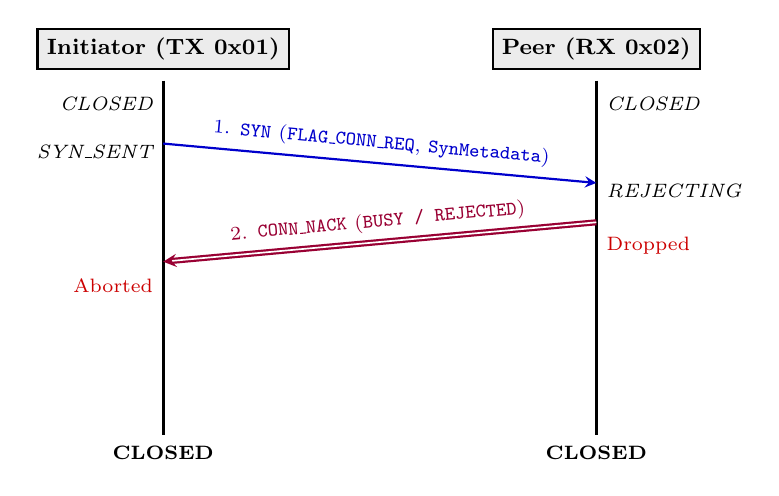
\begin{tikzpicture}[>=stealth, thick, font=\footnotesize]
    \draw[very thick] (0,0) -- (0,-4.5) node[below, font=\scriptsize\bfseries] {CLOSED};
    \draw[very thick] (5.5,0) -- (5.5,-4.5) node[below, font=\scriptsize\bfseries] {CLOSED};

    \node[draw, rectangle, fill=gray!15, minimum width=2.0cm, minimum height=0.5cm] at (0,0.4) {\textbf{Initiator (TX 0x01)}};
    \node[draw, rectangle, fill=gray!15, minimum width=2.0cm, minimum height=0.5cm] at (5.5,0.4) {\textbf{Peer (RX 0x02)}};

    \node[left, font=\scriptsize\itshape] at (0,-0.3) {CLOSED};
    \node[right, font=\scriptsize\itshape] at (5.5,-0.3) {CLOSED};
    \node[left, font=\scriptsize\itshape] at (0,-0.9) {SYN\_SENT};
    \node[right, font=\scriptsize\itshape] at (5.5,-1.4) {REJECTING};

    \draw[->, color=blue!80!black] (0,-0.8) -- (5.5,-1.3) node[midway, above, sloped, font=\scriptsize] {1. \texttt{SYN} (\texttt{FLAG\_CONN\_REQ}, \texttt{SynMetadata})};
    \draw[<-, color=purple!80!black, double] (0,-2.3) -- (5.5,-1.8) node[midway, above, sloped, font=\scriptsize] {2. \texttt{CONN\_NACK} (\texttt{BUSY / REJECTED})};

    \node[left, font=\scriptsize\color{red!80!black}] at (0,-2.6) {Aborted};
    \node[right, font=\scriptsize\color{red!80!black}] at (5.5,-2.1) {Dropped};
  \end{tikzpicture}%
  \label{fig:supp_seq_nack}%
}
\caption{Sequence interaction flows for 3-Way Handshake (3WHS) connection setup with dynamic metadata negotiation and rejection handling.}
\label{fig:supp_3whs_sequence}
\end{figure*}

\begin{figure}[htpb]
\centering
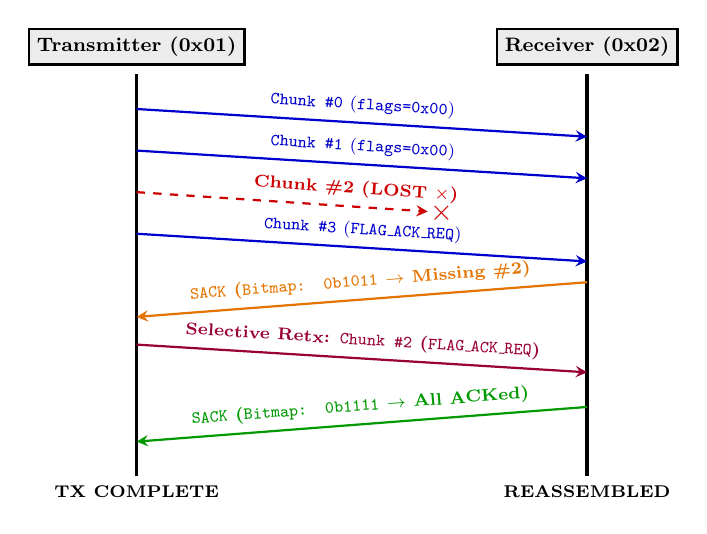
\begin{tikzpicture}[>=stealth, thick, font=\footnotesize, scale=0.88, transform shape]
  \draw[very thick] (0,0) -- (0,-5.8) node[below, font=\scriptsize\bfseries] {TX COMPLETE};
  \draw[very thick] (6.5,0) -- (6.5,-5.8) node[below, font=\scriptsize\bfseries] {REASSEMBLED};

  \node[draw, rectangle, fill=gray!15, minimum width=2.2cm, minimum height=0.5cm] at (0,0.4) {\textbf{Transmitter (0x01)}};
  \node[draw, rectangle, fill=gray!15, minimum width=2.2cm, minimum height=0.5cm] at (6.5,0.4) {\textbf{Receiver (0x02)}};

  % Initial Burst
  \draw[->, color=blue!80!black] (0,-0.5) -- (6.5,-0.9) node[midway, above, sloped, font=\scriptsize] {\texttt{Chunk \#0} (\texttt{flags=0x00})};
  \draw[->, color=blue!80!black] (0,-1.1) -- (6.5,-1.5) node[midway, above, sloped, font=\scriptsize] {\texttt{Chunk \#1} (\texttt{flags=0x00})};

  % Lost chunk #2
  \draw[->, color=red!80!black, dashed] (0,-1.7) -- (4.2,-1.98) node[near end, above, sloped, font=\scriptsize\bfseries] {\textbf{Chunk \#2 (LOST $\times$)}};
  \node[color=red!80!black, font=\large] at (4.4,-2.0) {$\mathbf{\times}$};

  % Chunk #3 with ACK_REQ
  \draw[->, color=blue!80!black] (0,-2.3) -- (6.5,-2.7) node[midway, above, sloped, font=\scriptsize] {\texttt{Chunk \#3} (\texttt{FLAG\_ACK\_REQ})};

  % SACK feedback (Bitmap 0b1011 = Chunks 0,1,3 received, 2 missing)
  \draw[<-, color=orange!90!black, thick] (0,-3.5) -- (6.5,-3.0) node[midway, above, sloped, font=\scriptsize\bfseries] {\texttt{SACK} (\texttt{Bitmap: 0b1011} $\rightarrow$ Missing \#2)};

  % Selective Retransmission of Chunk #2
  \draw[->, color=purple!80!black, thick] (0,-3.9) -- (6.5,-4.3) node[midway, above, sloped, font=\scriptsize\bfseries] {Selective Retx: \texttt{Chunk \#2} (\texttt{FLAG\_ACK\_REQ})};

  % Final SACK ACK
  \draw[<-, color=green!60!black, thick] (0,-5.3) -- (6.5,-4.8) node[midway, above, sloped, font=\scriptsize\bfseries] {\texttt{SACK} (\texttt{Bitmap: 0b1111} $\rightarrow$ All ACKed)};
\end{tikzpicture}
\caption{End-to-end data streaming flow, frame loss detection, and SACK-driven selective retransmission interaction.}
\label{fig:supp_data_transfer_sequence}
\end{figure}

\subsection{Transmitter Segmentation and SACK-ARQ Pipeline}
Algorithm~\ref{alg:supp_segmentation} details the formal transmission and selective retransmission logic executed by a LAMP transmitter across all operational modes.

\begin{algorithm}[htpb]
\caption{LAMP Payload Transmission and SACK-ARQ (Transmitter)}
\label{alg:supp_segmentation}
\footnotesize
\begin{algorithmic}[1]
\Require Payload $P$ (size $L > 0$), $dstAddr$, Chunk Size $S = S_{\max}$, Mode $M$
\Ensure Delivery Status (\texttt{OK} or \texttt{FAIL})
\State $N \gets \lceil L / S \rceil$
\If{$N > 255$} \State \Return \texttt{ERR\_PAYLOAD\_TOO\_LARGE} \EndIf
\State $msgId \gets \text{GetNextMsgId}()$
\For{$i \gets 0$ \textbf{to} $N-1$}
    \State $cLen \gets (i == N-1) ? (L - i \cdot S) : S$
    \State $flags \gets (M \in \{\text{Mode 3}, \text{Mode 4}\} \textbf{ and } i == N-1) ? \texttt{FLAG\_ACK\_REQ} : \texttt{0x00}$
    \State $hdr \gets \text{BuildHdr}(src, dst, msgId, N, i, cLen, flags)$
    \State $crc \gets \text{CalcCRC16}(hdr, P[i\cdot S : i\cdot S + cLen])$
    \State $F_i \gets \text{SerializeFrame}(hdr, P[i\cdot S : i\cdot S + cLen], crc)$
    \State $\text{Transmit}(F_i)$
\EndFor
\If{$M \in \{\text{Mode 1}, \text{Mode 2}\}$} \State \Return \texttt{OK} \Comment{Unreliable delivery complete} \EndIf
\State $retries \gets 0$; $poll \gets N-1$
\While{$retries \le R_{\mathrm{max}}$}
    \State $sack \gets \text{WaitForSack}(T_{\mathrm{timeout}})$
    \If{$sack == \text{TIMEOUT}$}
        \If{$retries == R_{\mathrm{max}}$} \State \textbf{break} \EndIf
        \State $\text{Transmit}(F_{poll})$ \textbf{with} \texttt{FLAG\_ACK\_REQ}; $retries \gets retries + 1$
    \ElsIf{$\text{IsAllAcked}(sack.bitmap)$}
        \State \Return \texttt{OK} \Comment{Full payload delivery confirmed}
    \Else
        \If{$retries == R_{\mathrm{max}}$} \State \textbf{break} \EndIf
        \State $missing \gets \text{MissingChunks}(sack.bitmap)$
        \For{$idx \in missing$}
            \State $cLen \gets (idx == N-1) ? (L - idx \cdot S) : S$
            \State $flags \gets (idx == \text{Last}(missing)) ? \texttt{FLAG\_ACK\_REQ} : \texttt{0x00}$
            \State $hdr \gets \text{BuildHdr}(src, dst, msgId, N, idx, cLen, flags)$
            \State $crc \gets \text{CalcCRC16}(hdr, P[idx\cdot S : idx\cdot S + cLen])$
            \State $F_{idx} \gets \text{SerializeFrame}(hdr, P[idx\cdot S : idx\cdot S + cLen], crc)$
            \State $\text{Transmit}(F_{idx})$
        \EndFor
        \State $poll \gets \text{Last}(missing)$; $retries \gets retries + 1$
    \EndIf
\EndWhile
\State \Return \texttt{ERR\_MAX\_RETRIES\_EXCEEDED}
\end{algorithmic}
\end{algorithm}

\subsection{Adaptive SACK Timeout Parameters}
Table~\ref{tab:supp_timeouts} details representative timeout parameters across spreading factors (BW~125~kHz, CR~4/5).

\begin{table}[htpb]
\centering
\caption{Adaptive SACK Timeout Values (BW~125~kHz, CR~4/5, 8-symbol preamble, explicit header, PHY CRC on; 255-byte data frame, 14-byte SACK for $N=20$ chunks)}
\label{tab:supp_timeouts}
\renewcommand{\arraystretch}{1.15}
\footnotesize
\resizebox{\columnwidth}{!}{%
\begin{tabular}{|c|r|r|r|r|}
\hline
\textbf{SF} & \textbf{$\widehat{T}_{\mathrm{DATA}}$ (ms)} & \textbf{$\widehat{T}_{\mathrm{SACK}}$ (ms)} & \textbf{$\alpha(\widehat{T}_{\mathrm{DATA}}+\widehat{T}_{\mathrm{SACK}})+\delta$ (ms)} & \textbf{$T_{\mathrm{timeout}}$ (ms)} \\ \hline
7  &  400 &   46 &   719 & 1000 \\ \hline
8  &  707 &   82 &  1234 & 1234 \\ \hline
9  & 1250 &  165 &  2173 & 2173 \\ \hline
10 & 2296 &  289 &  3927 & 3927 \\ \hline
11 & 5001 &  660 &  8541 & 8541 \\ \hline
12 & 9019 & 1155 & 15312 & 15312 \\ \hline
\end{tabular}}
\end{table}

\section{Extended Simulation Studies: Blocks F, G, and H}
\label{sec:supp_sim}

\subsection{Block F: Message Size Scaling (10~B to 62.2~kB)}
Block~F evaluates protocol performance under large payload scaling at SF7 across message sizes $N \in \{20, 50, 100, 255\}$ chunks of 244~B (4.9 to 62.2~kB, reaching the maximum capacity of a single LAMP session). Comparative baselines include Stop-and-Wait, MPLR~\cite{mplr-chen2019}, and LoRaMesher~\cite{sole2026largetransfer}.

Fig.~\ref{fig:supp_ns3_size} depicts the 90\% PDR delivery range in the Urban channel and goodput under static lossless conditions. The delivery range of LAMP remains invariant to message size (Mode~4 maintains 4.13~km; Mode~3 maintains 4.56~km up to 100 chunks and 4.13~km at 255 chunks). Conversely, architectures assigning individual per-frame retry budgets experience compounding degradation as $N$ increases: Stop-and-Wait drops from 3.38~km to 2.26~km, while LoRaMesher ($R=10$) falls from 4.13~km to 3.09~km.

For MPLR, behavior depends on the interpretation of its retry budget: if $R_{\mathrm{max}}$ applies globally across the entire multi-batch transfer, range collapses to 3.7~km at $N=50$ and fails to reach 90\% at $N=255$. If $R_{\mathrm{max}}$ is refreshed per batch of 40 frames, MPLR maintains 4.13~km, matching Mode~4. Under this favorable reading, LAMP retains higher goodput due to its compact 9-byte header (+3\% faster at 62.2~kB, delivering in 103~s vs. 106~s).

\begin{figure*}[t]
\centering
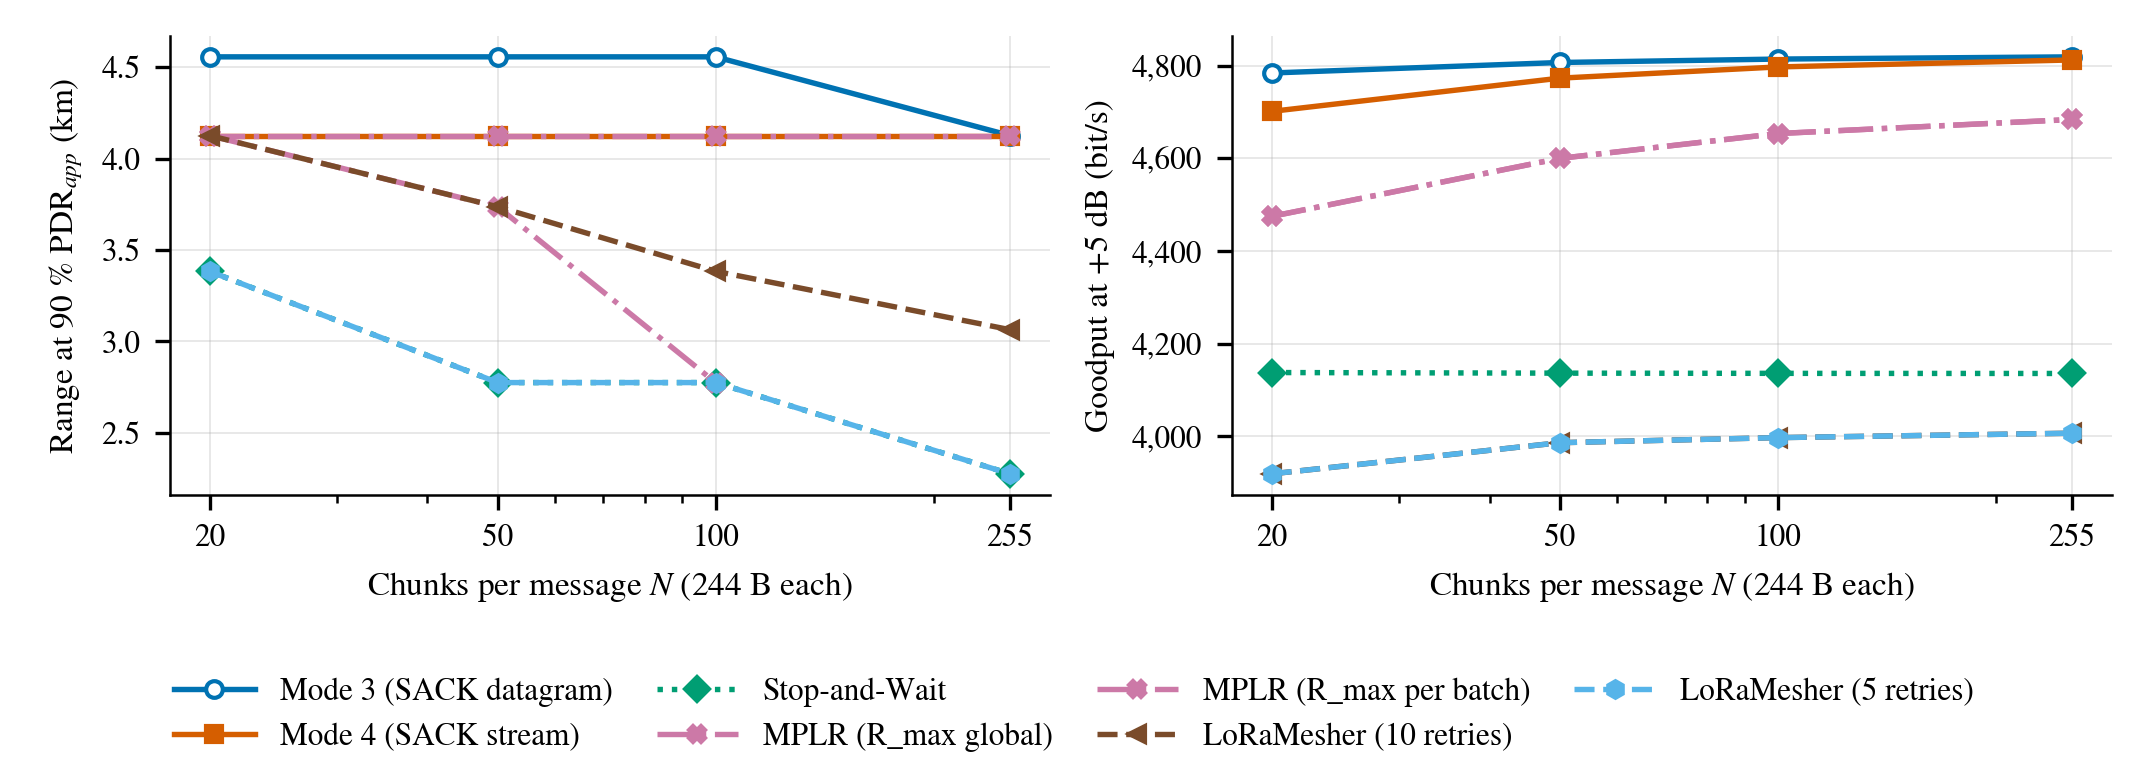
\includegraphics[width=0.92\textwidth]{img/ns3_range_goodput_vs_n.png}
\caption{Urban range (largest distance with mean $PDR_{\mathrm{app}} \ge 90\%$) and goodput at +5~dB (static channel) versus the number of 244-byte chunks per message, SF7, 50 seeds. MPLR is evaluated under both global retry budget and per-batch refresh.}
\label{fig:supp_ns3_size}
\end{figure*}

\subsection{Block G: Asymmetric SACK Feedback Loss Robustness}
Block~G investigates performance when feedback frames (SACK, SYN-ACK, ACK) are subjected to loss probability $p_{\mathrm{ack}} \in \{0, 20, 40\}\%$, concurrent with data frame loss $p \in [0, 50]\%$ (SF7, $N=20$).

Because lost SACK feedback triggers the timer-driven poll mechanism, the penalty is predominantly manifested as latency rather than transfer aborts. At $p=20\%$ and $p_{\mathrm{ack}}=20\%$, Mode~3 maintains 98\% transfer completion, with elapsed time increasing moderately from 11.1~s to 11.7~s; at $p_{\mathrm{ack}}=40\%$, completion remains at 92\% (13.1~s). In Mode~4, lost SYN-ACK frames incur handshake retries, increasing latency to 15.8~s at $p=20\%, p_{\mathrm{ack}}=40\%$.

In contrast, Stop-and-Wait exhibits severe sensitivity to feedback losses: at $p=30\%$, its completion rate plunges from 100\% (lossless feedback) down to 84\% at $p_{\mathrm{ack}}=20\%$ and 46\% at $p_{\mathrm{ack}}=40\%$, whereas LAMP Mode~3 preserves 90\% and 76\% completion under the same harsh feedback loss regimes.

\subsection{Block H: Retransmission Timeout and Poll Rule Ablation}
Block~H isolates the architectural benefit of the LAMP timeout poll rule (which retransmits the final chunk carrying \texttt{FLAG\_ACK\_REQ} upon SACK expiration, rather than restarting full-window retransmission). Without this targeted poll rule, Mode~3 completion drops drastically under high frame loss: at $p=30\%$, completion falls from 92\% to 80\%; at $p=40\%$, completion plummets from 56\% to 40\%. This confirms that targeted polling prevents catastrophic retry exhaustion.

\subsection{Rural, Water, and Static Propagation Comparisons}
For completeness, Figs.~\ref{fig:supp_rural}, \ref{fig:supp_water}, and \ref{fig:supp_static} provide the detailed comparative performance curves of LAMP against MPLR, LoRaMesher, and Stop-and-Wait across Rural, Water, and Static AWGN channel environments, complementing the Urban channel results reported in the main manuscript.

\begin{figure*}[htpb]
\centering
\subfloat[Rural Propagation Channel]{%
  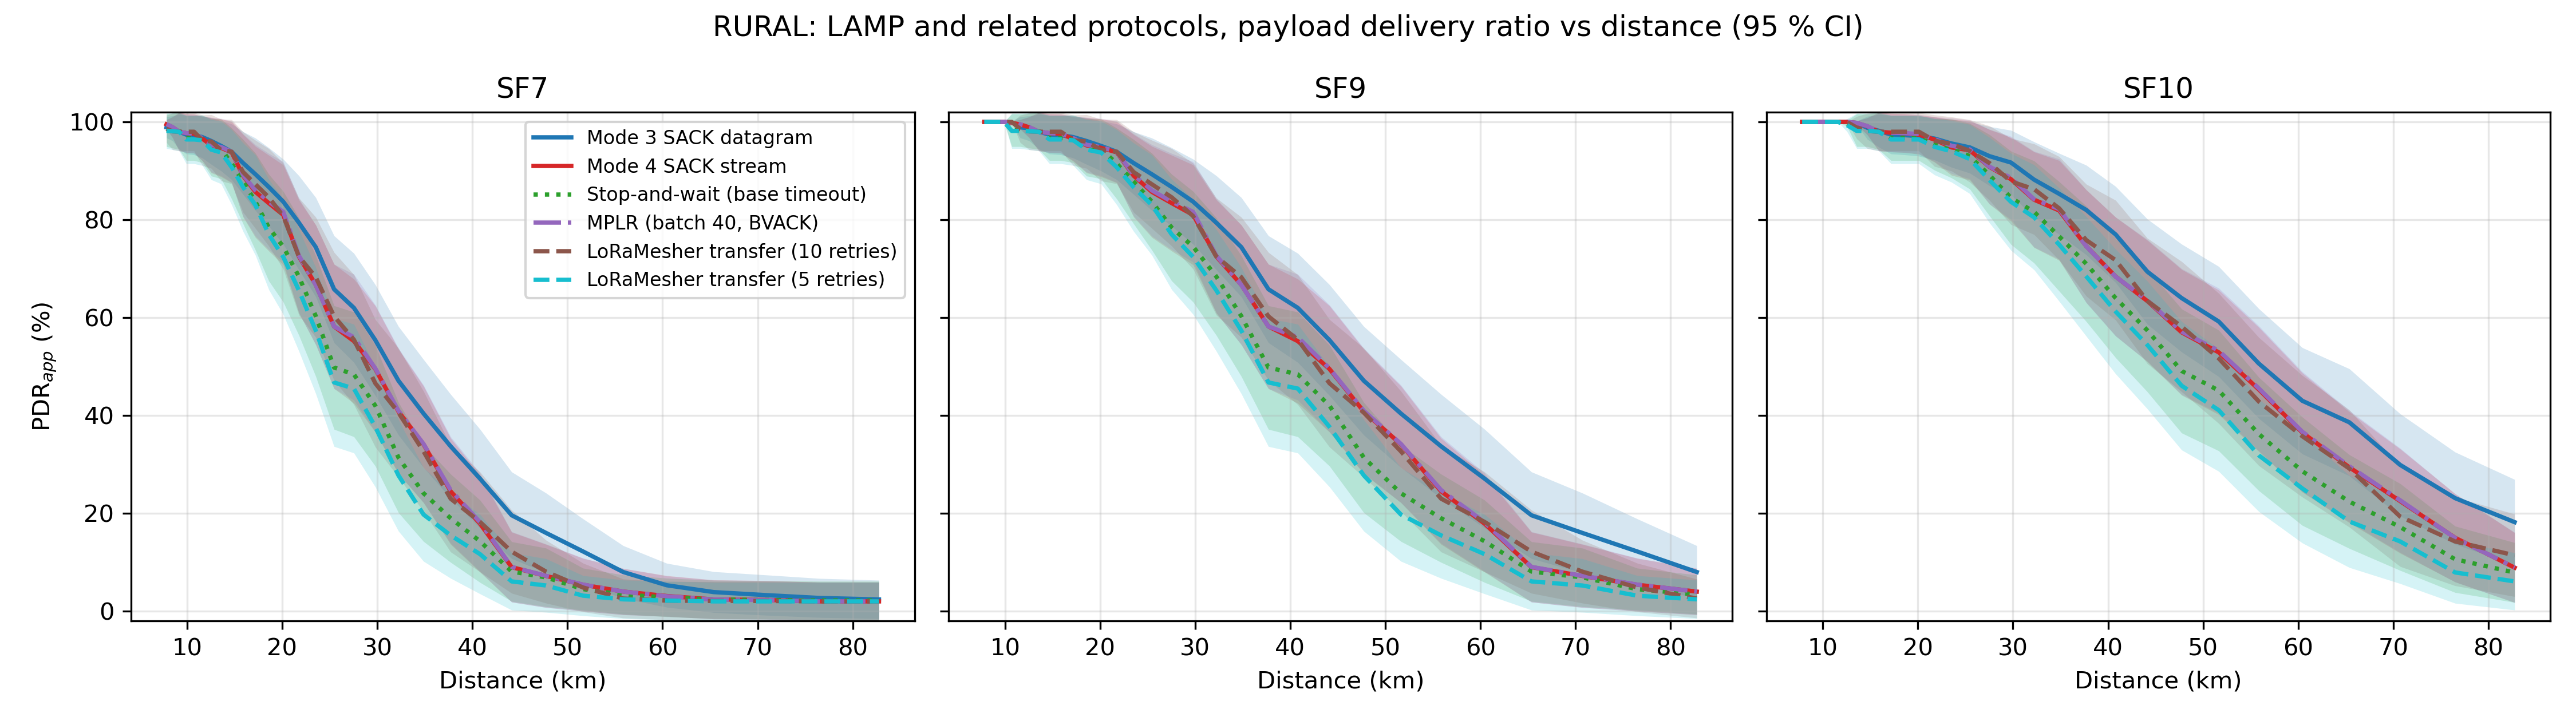
\includegraphics[width=0.485\textwidth]{img/ns3_pdr_distance_rural_related.png}%
  \label{fig:supp_rural}%
}\hfill
\subfloat[Water Propagation Channel]{%
  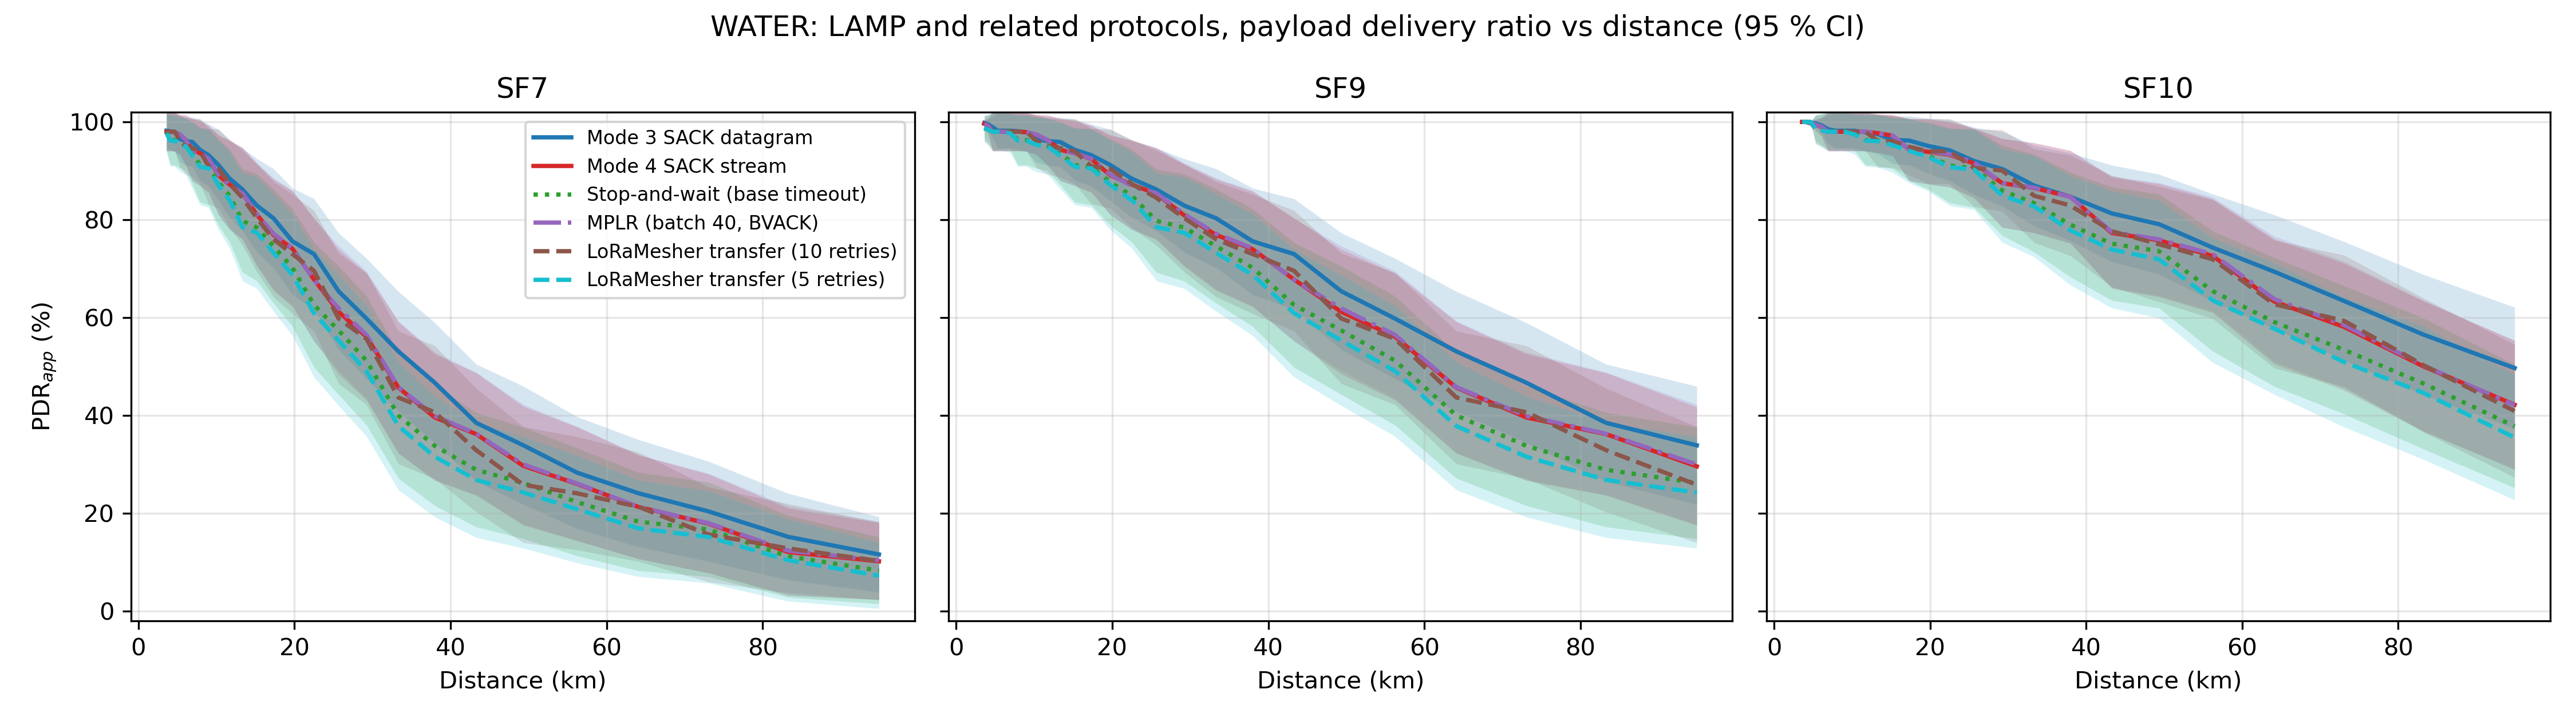
\includegraphics[width=0.485\textwidth]{img/ns3_pdr_distance_water_related.png}%
  \label{fig:supp_water}%
}
\caption{$PDR_{\mathrm{app}}$ versus distance across alternative propagation environments for LAMP and related protocols (SF7, 50 seeds, 90\% PDR threshold marked with dotted line).}
\label{fig:supp_rural_water}
\end{figure*}

\begin{figure*}[htpb]
\centering
\subfloat[PDR vs. Nominal SNR in Static Channel]{%
  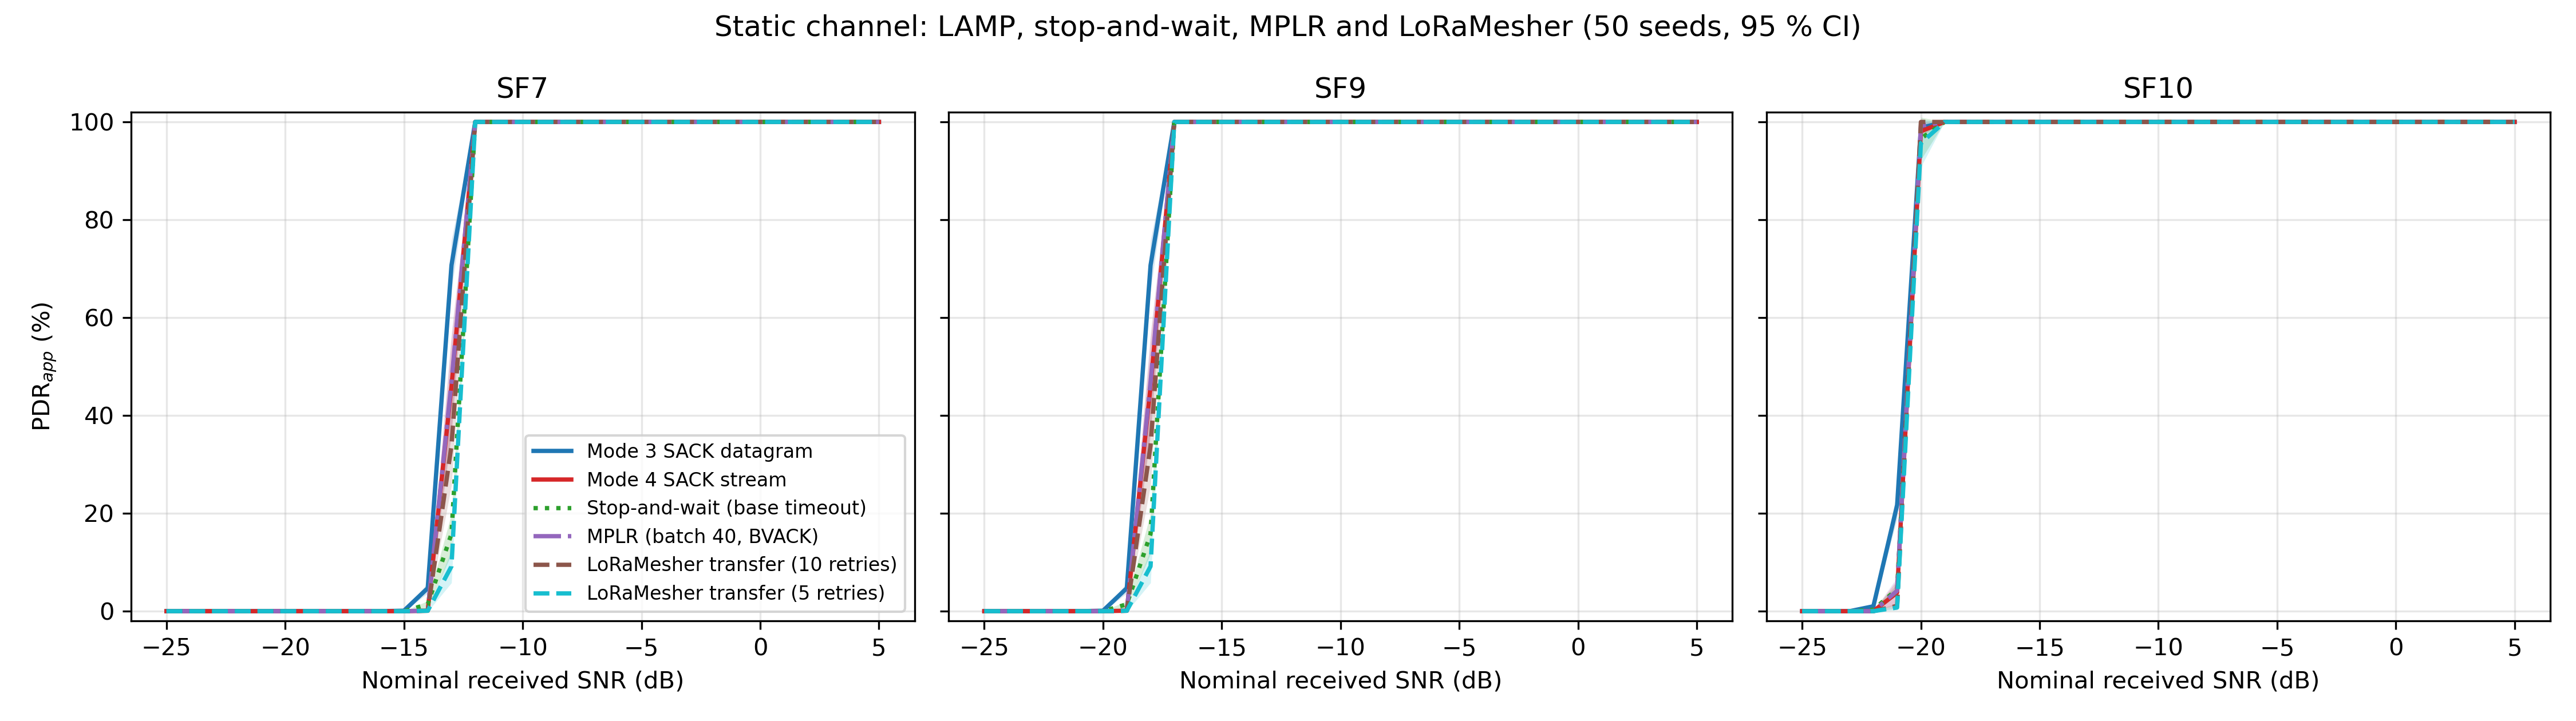
\includegraphics[width=0.485\textwidth]{img/ns3_pdr_snr_related.png}%
  \label{fig:supp_static_pdr}%
}\hfill
\subfloat[Goodput vs. Nominal SNR in Static Channel]{%
  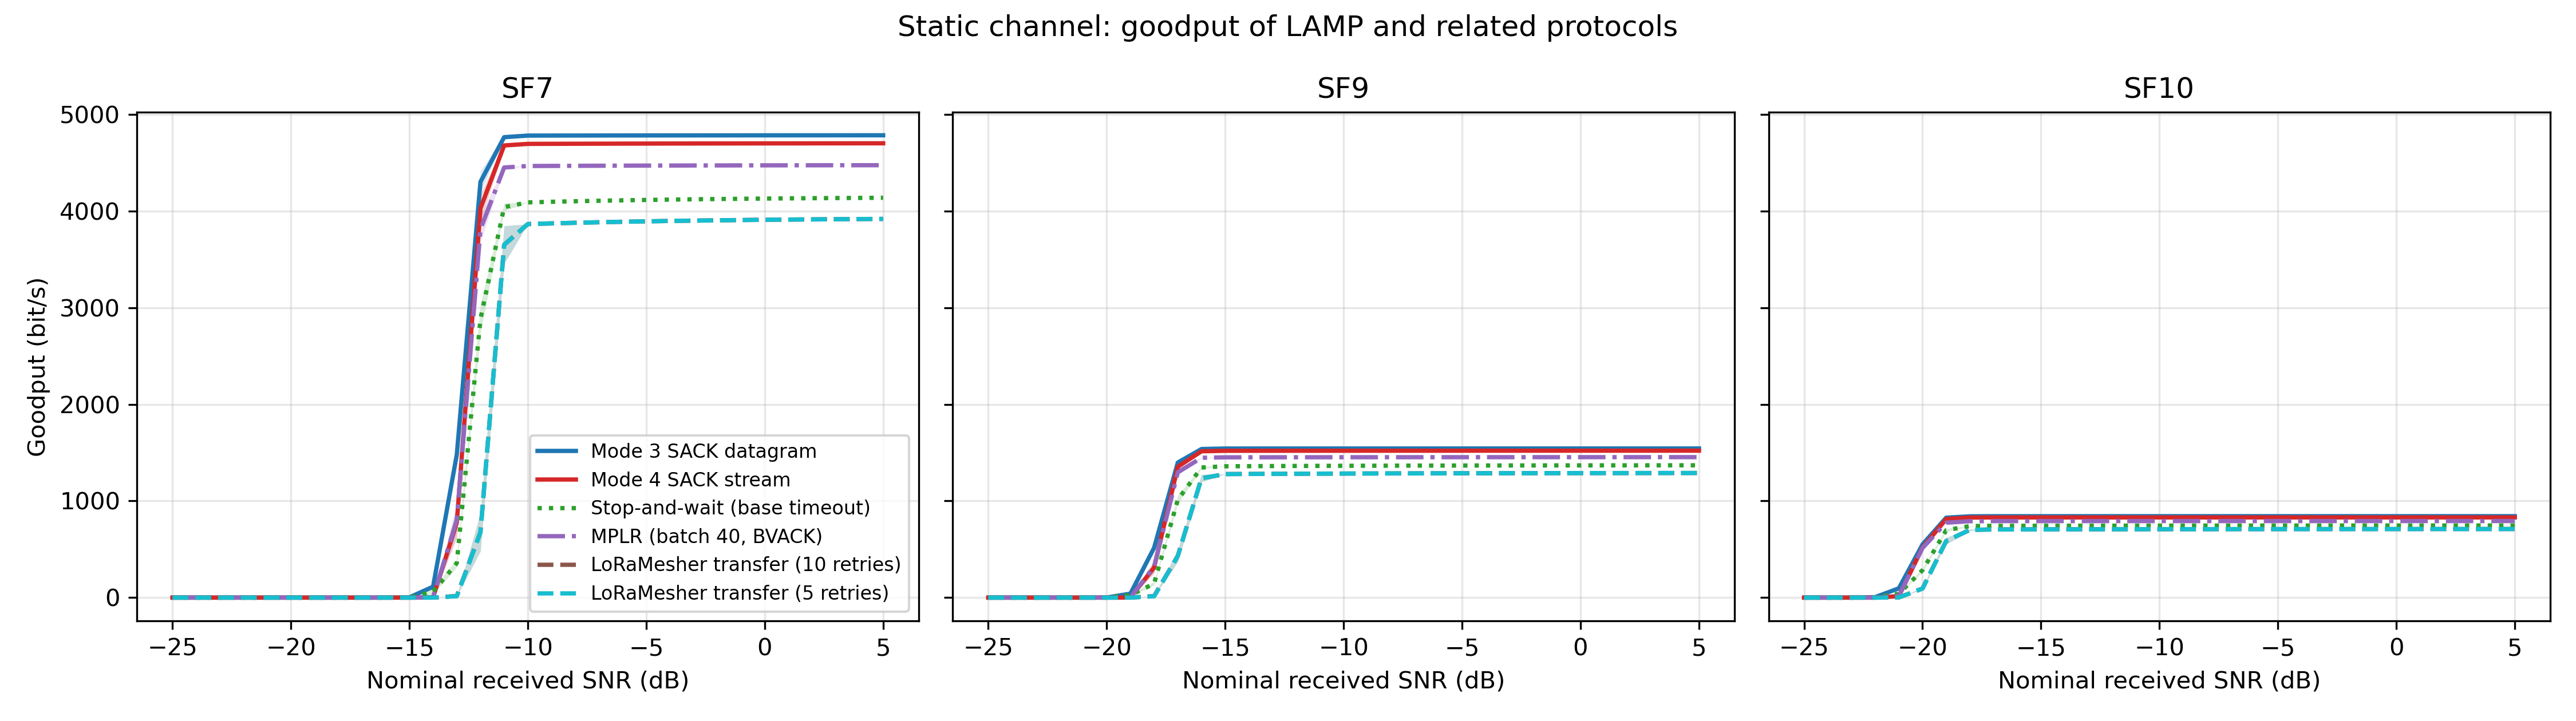
\includegraphics[width=0.485\textwidth]{img/ns3_goodput_snr_related.png}%
  \label{fig:supp_static_goodput}%
}
\caption{Performance comparison under Static AWGN conditions versus nominal SNR for LAMP and related protocols (SF7, 4.88~kB transfer, 50 seeds).}
\label{fig:supp_static}
\end{figure*}

\bibliographystyle{IEEEtran}
\bibliography{paper}

\end{document}
